
\addtocontents{toc}{\vspace{\baselineskip}APPENDICES}
\setcounter{table}{0}
\renewcommand{\thetable}{\Alph{chapter}\arabic{table}}
\GrizzAppendix{Tables and Figures} \label{ch:extra}

\begin{sidewaystable}
\caption{Geographic information of sampling points at each  surveyed lakes }
\label{tab:Surveyed Lakes}
\begin{center}
\scalebox{0.86}{
\begin{tabular}{lllrrl}
\hline \\
\multicolumn{1}{c}{Name of Lake} & \multicolumn{1}{c}{Shorten Code} & \multicolumn{1}{c}{County} & \multicolumn{1}{c}{Longitude} & \multicolumn{1}{c}{Latitude} &
\multicolumn{1}{c}{HUC 14 Reachcode} \\ \hline
Bear Lake & BEA & Kalkaska & -84.9438079727 & 44.7286139551 & 04060103001048 \\
Belleville Lake & BEL & Wayne & -83.4663770506 & 42.2145253455 & 04090005001822 \\
Bogie Lake & BOG & Oakland & -83.5054334514 & 42.6188513679 & 04090005001348 \\
Brighton Lake & BRI & Livingston & -83.7958137995 & 42.5169054061 & 04090005001500 \\
Coldwater Lake & COL & Isabella & -84.9565922285 & 43.6613607551 & 04080202000902 \\
Deer Lake & DEE & Charlevoix & -84.9770123186 & 45.166441811 & 04060105001116 \\
Ford Lake & FOR & Washtenaw & -83.5849122567 & 42.2159133043 & 04090005001823 \\
Houghton Lake & HOU & Roscommon & -84.7262816343 & 44.3385407778 & 04060102002461 \\
Hudson Lake & HUD & Lenawee & -84.2545514803 & 41.835000535 & 04100002001317 \\
Intermediate lake & INT & Antrim & -85.2293359783 & 45.0265435299 & 04060105003435 \\
Lake Cadillac & CAD & Wexford & -85.4266252378 & 44.2410192547 & 04060102001951 \\
Lake Margrethe & MAR & Crawford & -84.7830175986 & 44.6464747348 & 04060103001058 \\
Lake Nepessing & NEP & Lapeer & -83.3728265865 & 43.0161554865 & 04080204001601 \\
Lime Lake & LIM & Hillsdale & -84.3791188315 & 41.7861576065 & 04100006000872 \\
Little Glen Lake & LGL & Leelanac & -85.963633169 & 44.8687577197 & 04060104000456 \\
Little Round Lake & LRO & Lenawee & -84.3527742524 & 41.9093334799 & 04100006000858 \\
Manitou Lake & MAN & Shiawassee & -84.2038069227 & 42.925537136 & 04050005000939 \\
Ore Lake & ORE & Livingston & -83.7959940227 & 42.4805569493 & 04090005001574 \\
Paradise Lake & PAR & Emmett & -84.7512093045 & 45.6872890124 & 04060105001063 \\
Platte Lake & PLA & Benzie & -86.092789204 & 44.6900468421 & 04060104000558 \\
Pontiac Lake & PON & Oakland & -83.451096479 & 42.6664394508 & 04090005001288 \\
Posey lake & POS & Lenawee & -84.3007962072 & 41.8970465491 & 04100006000857 \\
Round Lake & ROU & Lenawee & -84.1318219224 & 42.0712488438 & 04100002001130 \\
Sanford Lake & SAN & Midland & -84.3860517762 & 43.7104273774 & 04080201001468 \\
Silver Lake & SIL & Grand Traverse & -85.687150728 & 44.6980286859 & 04060105003542 \\
Stony Creek Lake & STO & Oakland & -83.0870627175 & 42.7260717429 & 04090003001029 \\
Sugden Lake & SUG & Oakland & -83.4972563639 & 42.6173106359 & 04090005001347 \\
West Twin Lake & WTL & Montmorency & -84.3501403918 & 44.8762035424 & 04070007001271 \\
Wixom Lake & WIX & Gladwin & -84.3537506311 & 43.8276751177 & 04080201001442 \\ \hline
\multicolumn{3}{r}{{HUC=Hydrological Unit Code}} \\ \hline
\multicolumn{3}{r}{{GPS Coordinates are in decimal degrees, North American Datum of 1983 (NAD83)}} \\ \hline
\end{tabular}}
\end{center}
\end{sidewaystable}

\begin{center}
\begin{longtable}{p{3.5cm}p{1cm}p{3.3cm}}
\caption{Table Summary} \label{tab:variables} \\
\hline \multicolumn{1}{l}{\textbf{Measured Variable (Units)}} &
\multicolumn{1}{l}{\textbf{Shortened Code Name}} &
\multicolumn{1}{l}{\textbf{Transformation}} \\
\hline
\endfirsthead
\multicolumn{3}{c}%
{{\bfseries \tablename\ \thetable{}  -- continued from previous page}} \\
\hline
\multicolumn{1}{l}{\textbf{Measured Variable (Units)}} &
\multicolumn{1}{l}{\textbf{Shortened Code Name}} &
\multicolumn{1}{l}{\textbf{Transformation}} \\
\hline
\endhead
\hline \multicolumn{3}{r}{{Continued on next page}} \\ \hline
\endfoot
\hline
\hline
\endlastfoot
Total microcysin of all 12 congeners ($\mu$g/L) & SUM &  $log10$(SUM+0.03) \\
Cyano \emph{16s rRNA} gene copies (cp/L) & X16SRNA &  $log10$(X16SRNA+45) \\
\emph{mcyE} gene copies (cp/L) & MCYE &  $log10$(MCYE+45) \\
Ortho-P (mg-P/L) & OP & $log10$(OP+0.003) \\
Nitrate/Nitrite (mg-N/L) & NO3 &  $log10$(NO3+0.04) \\
Ammonia (mg-N/L) & NH3 & $log10$(NH3+0.006) \\
Total nitrogen (mg-N/L) & TN & $log10$(TN+0.116) \\
Total Kjeldahl nitrogen (mg-N/L) & TKN & $log10$(TKN+0.07) \\
Total phosphorus (mg-P/L) & TP & $log10$(TP+0.002) \\
Total nitrogen to total phosphorus ratio & TNTP &  None \\
Measured pH of Lake & pH & None \\
Dissolved oxygen (mg/L) & DO &  $log10$(do+0.01) \\
Conductance (uS/cm) & conduc &  $log10$(conduc+0.01) \\
Turbidity (NTU) & turb &  $log10$(turb+0.01) \\
Chloraphyll-a (RFU) & chloro & $log10$(chloro+0.01) \\
Phycocyanin (RFU) & phyco &  $log10$(phyco+0.01) \\
Maximum depth of lake (meters) &   Max\_Depth &  None \\
Lake area (sq Km) & LkArea & $log10$(LkArea+1) \\
Watershed Area (sq Km) &  WtWhArea & $log10$(WtWhArea+1) \\
Lake area to watershed area ratio & LkWshRatio &  $log10$(LkWshRatio+1) \\
Water Land-Use (\%) & Water &  None \\
Developed Land-Use  (\%) & Developed & None \\
Barren Land-Use (\%) & Barren & None \\
Forest Land-Use (\%) & Fores & None \\
Shrubs Land-Use (\%) & Shrubs & None \\
Herbaceous Land-Use (\%) & Herbaceous  & None \\
Agriculture Land-Use (\%) & Agriculture & None \\
Wetlands Land-Use (\%) & Wetlands & None \\
Average precipitation 3 days prior (mm) & precip3 &  $log10$(precip3+1) \\
Average precipitation 5 days prior (mm)  & precip5 & $log10$(precip5+1) \\
Average precipitation 7 days prior (mm) & precip7 &  $log10$(precip7+1) \\
Average precipitation 30 days prior (mm) & precip30 &  $log10$(precip30+1) \\
Water temperature at time of sampling (Celcius) & wtemp & None \\
Average temperature 3 days prior from GHCN (Celcius) & temp3&  None \\
Average temperature 5 days prior from GHCN (Celcius) & temp5 & None \\
Average temperature 7 days prior  from GHCN (Celcius) &  temp7 & None \\
Average temperature 30 days prior from GHCN (Celcius) & temp30 &  None \\
Average Temperature from Hobo pendant 30 days prior (Celcius) & hobotemp & None \\
Average light intensity from Hobo pendant days prior (lux) & hobolight & $log10$(hobolight+1) \\
Zebra mussel Mass (grams) & MusselMass &  $log10$(MusselMass+1) \\
Zebra mussel (counts) &  MusselNum & $log10$(MusselNum+1) \\
\hline
\end{longtable}
\end{center}

\begin{figure}
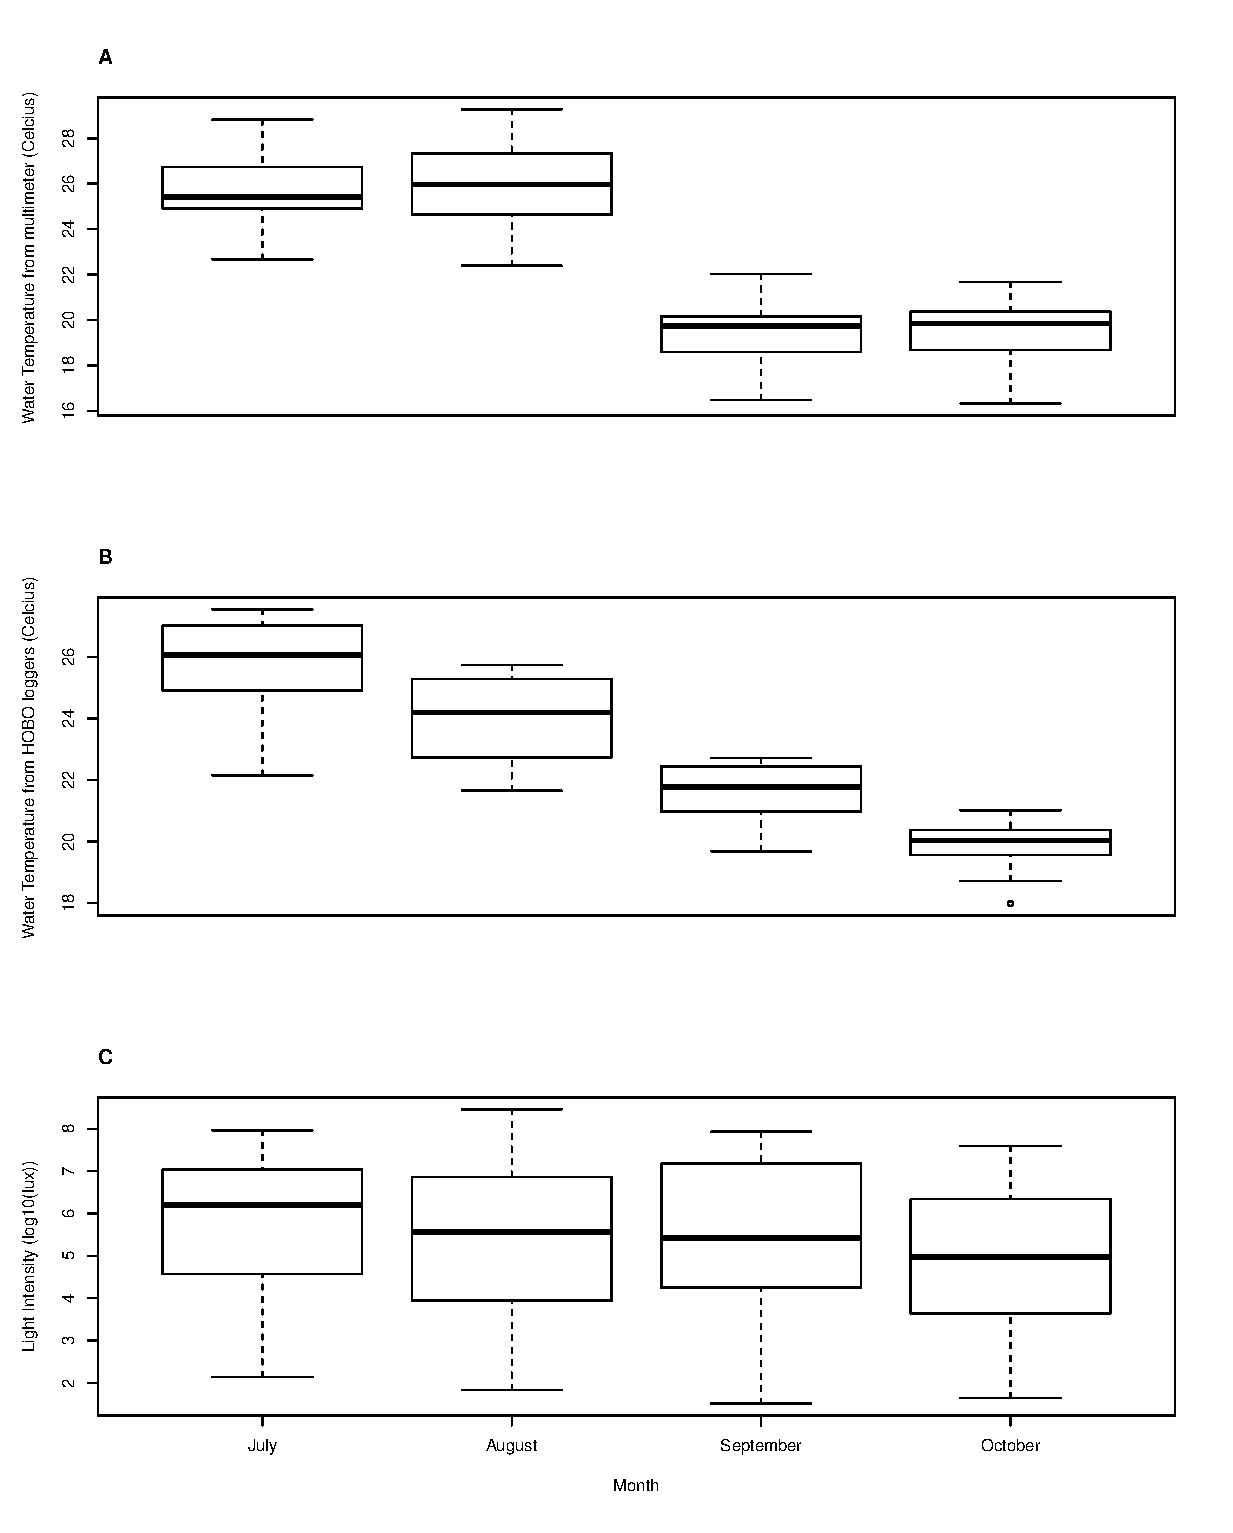
\includegraphics[width=\textwidth]{figures/hobo}
\caption{
(A): Boxplot summary of the average lake temperature measured at the time of sampling with hand-held multimeter 
(B): Boxplot summary of average lake temprature from HOBO loggers. 
(C): Boxplot summary of light intensity also measured by HOBO loggers.
} 
\label{fig:hobo}
\end{figure}


\begin{figure}[!h]
 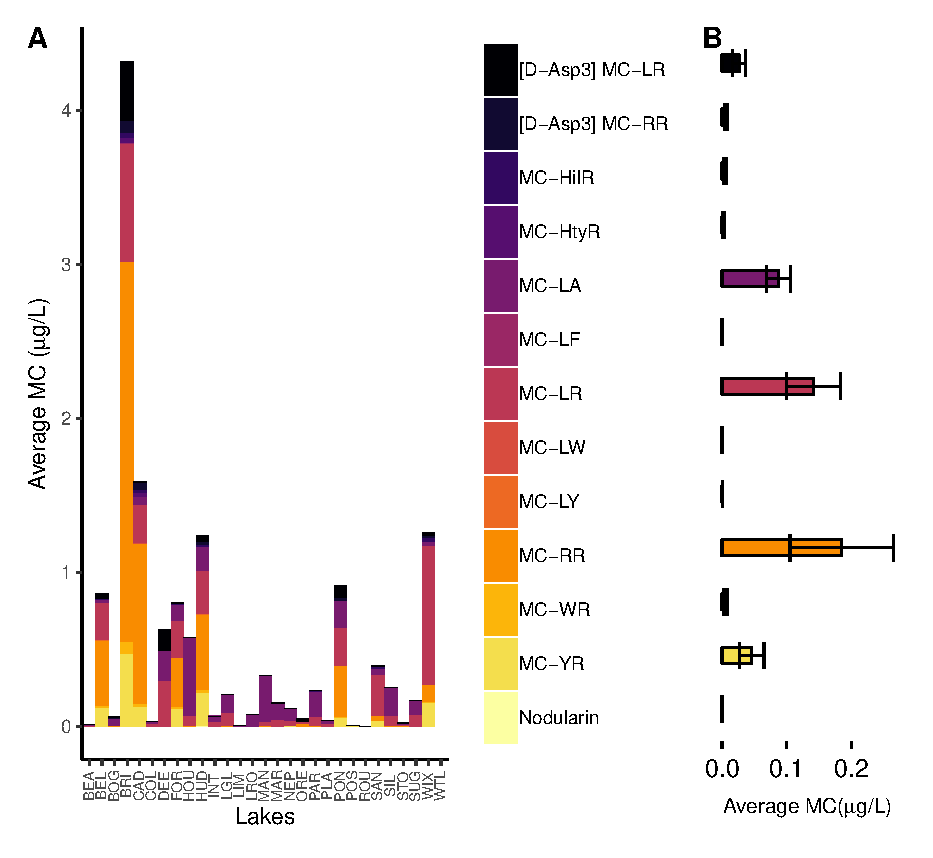
\includegraphics[width=\textwidth]{figures/congenerbar}
 \caption{
 (A): Average MC found at each lake in all four months. The height of each bar represents the total average of MC. The proportion of each congener is represented by color in each bar  
(B): Average MC congener with the included error bars represents one standard deviation of the mean}
 \label{fig:congenerbar}
\end{figure}



\begin{figure}[!ht]
\scalebox{1.14}{
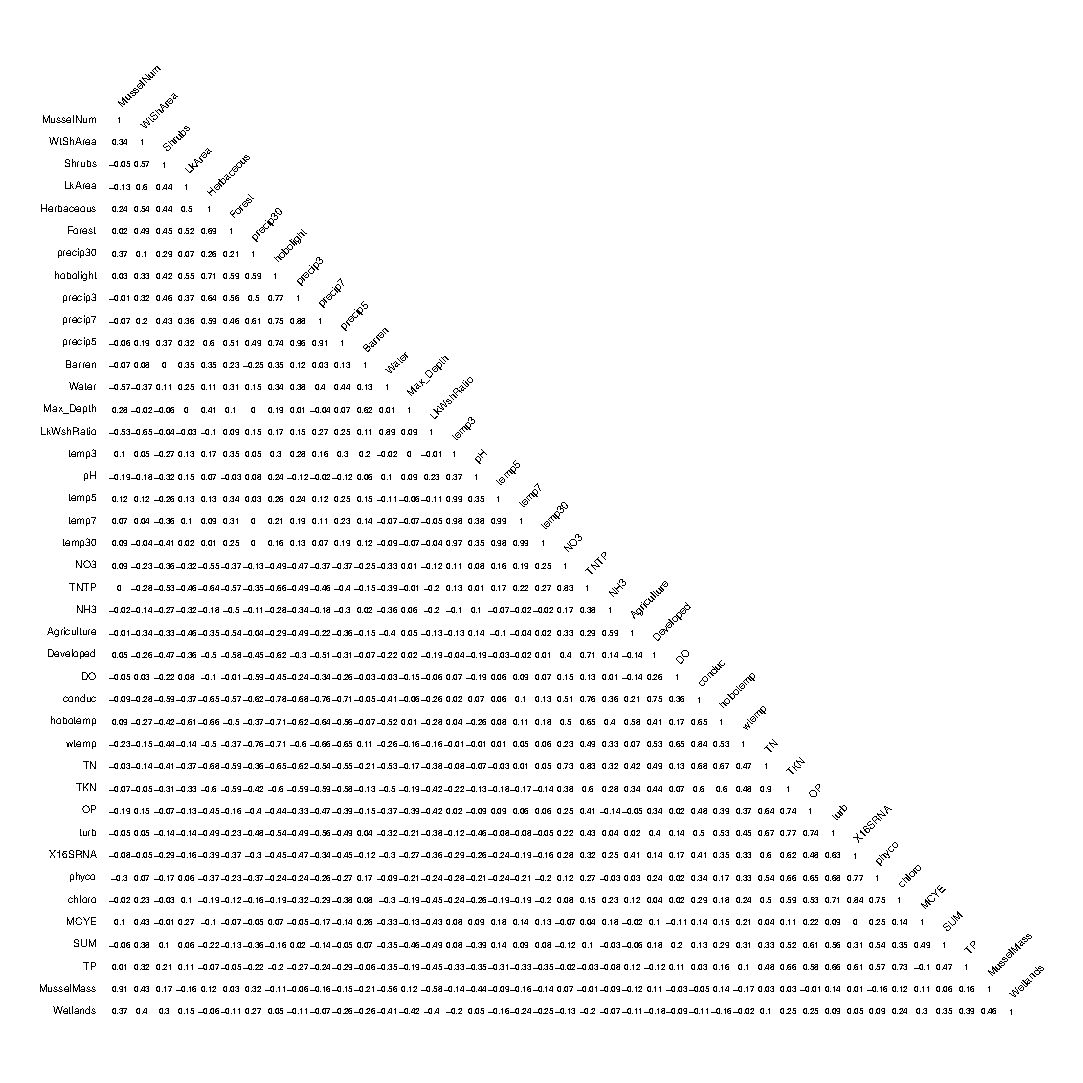
\includegraphics[width=\textwidth]{figures/matrixfull}}
\caption{Correlation matrix displaying Pearson's coefficient on the full data.}
\label{fig:matrixfull}
\end{figure}


\begin{figure}[!hp]
\centering
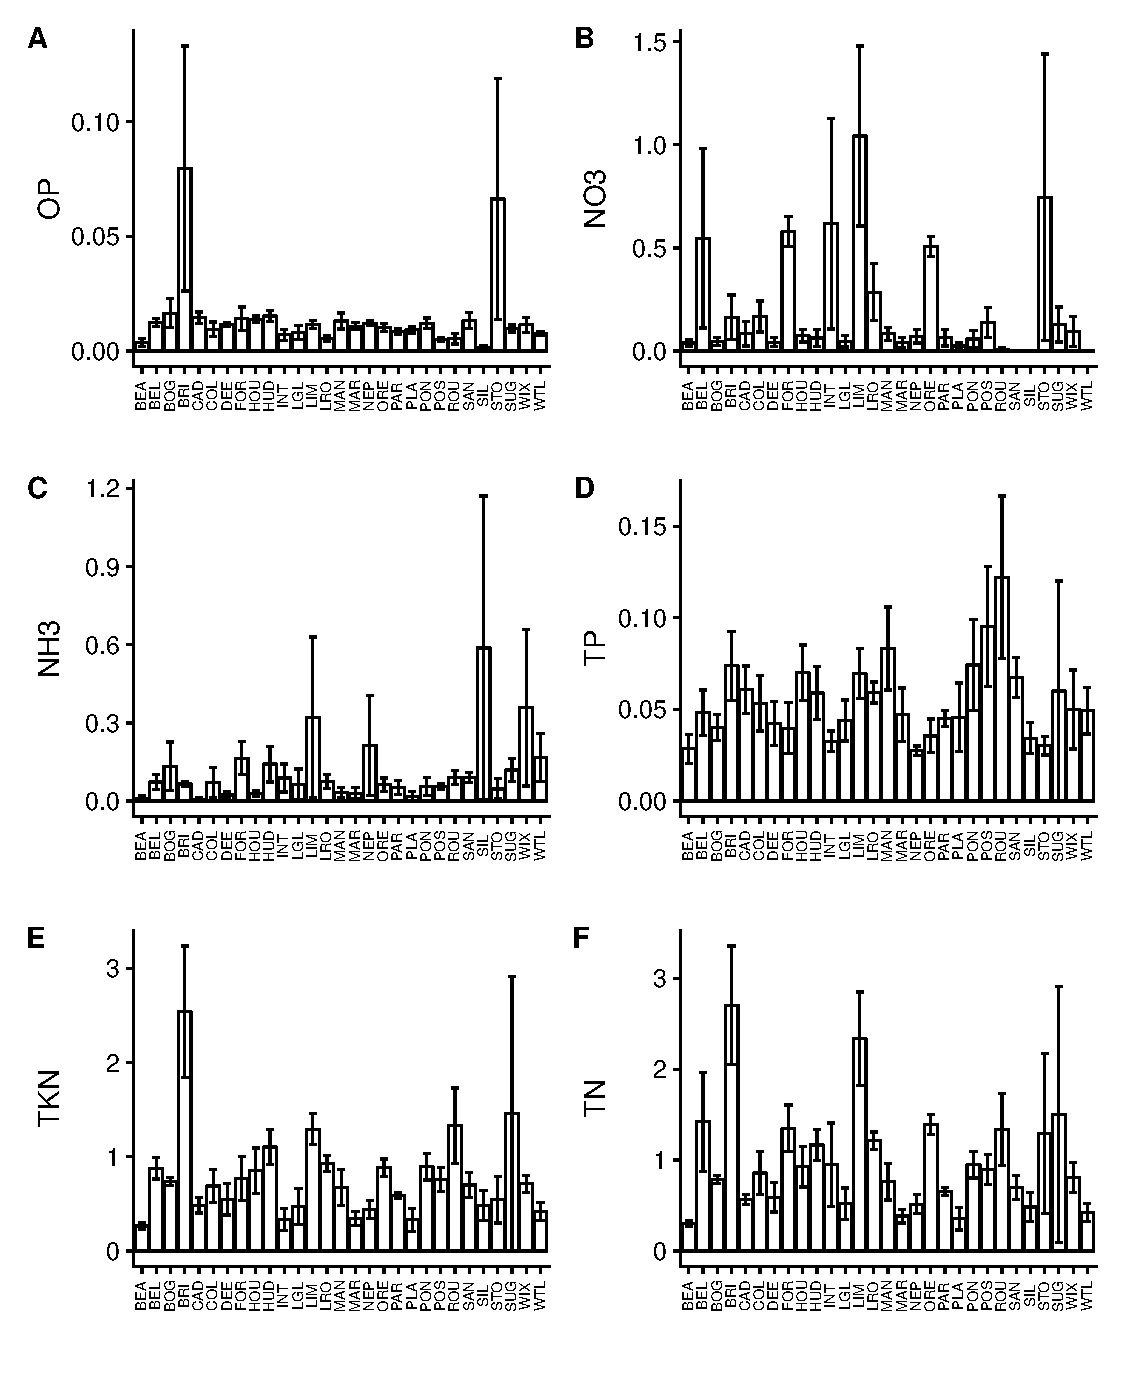
\includegraphics[width=\textwidth]{figures/nutboxplotlake}
\caption{Average nutrient concentrations for each lake for all of summer 2017. Figure (A): Orthophosphate (mg-P/L). Figure (B): Nitrate+nitrite (mg-N/L). Figure (C): Ammonia (mg-N/L). Figure (D): Total phosphorus (mg-P/L). Figure (E): Total Kjeldahl nitrogen (mg-N/L). Error bars represents one standard deviation of the mean. }
\label{fig:nutrients}
\end{figure}


\begin{figure}[!hp]
\centering
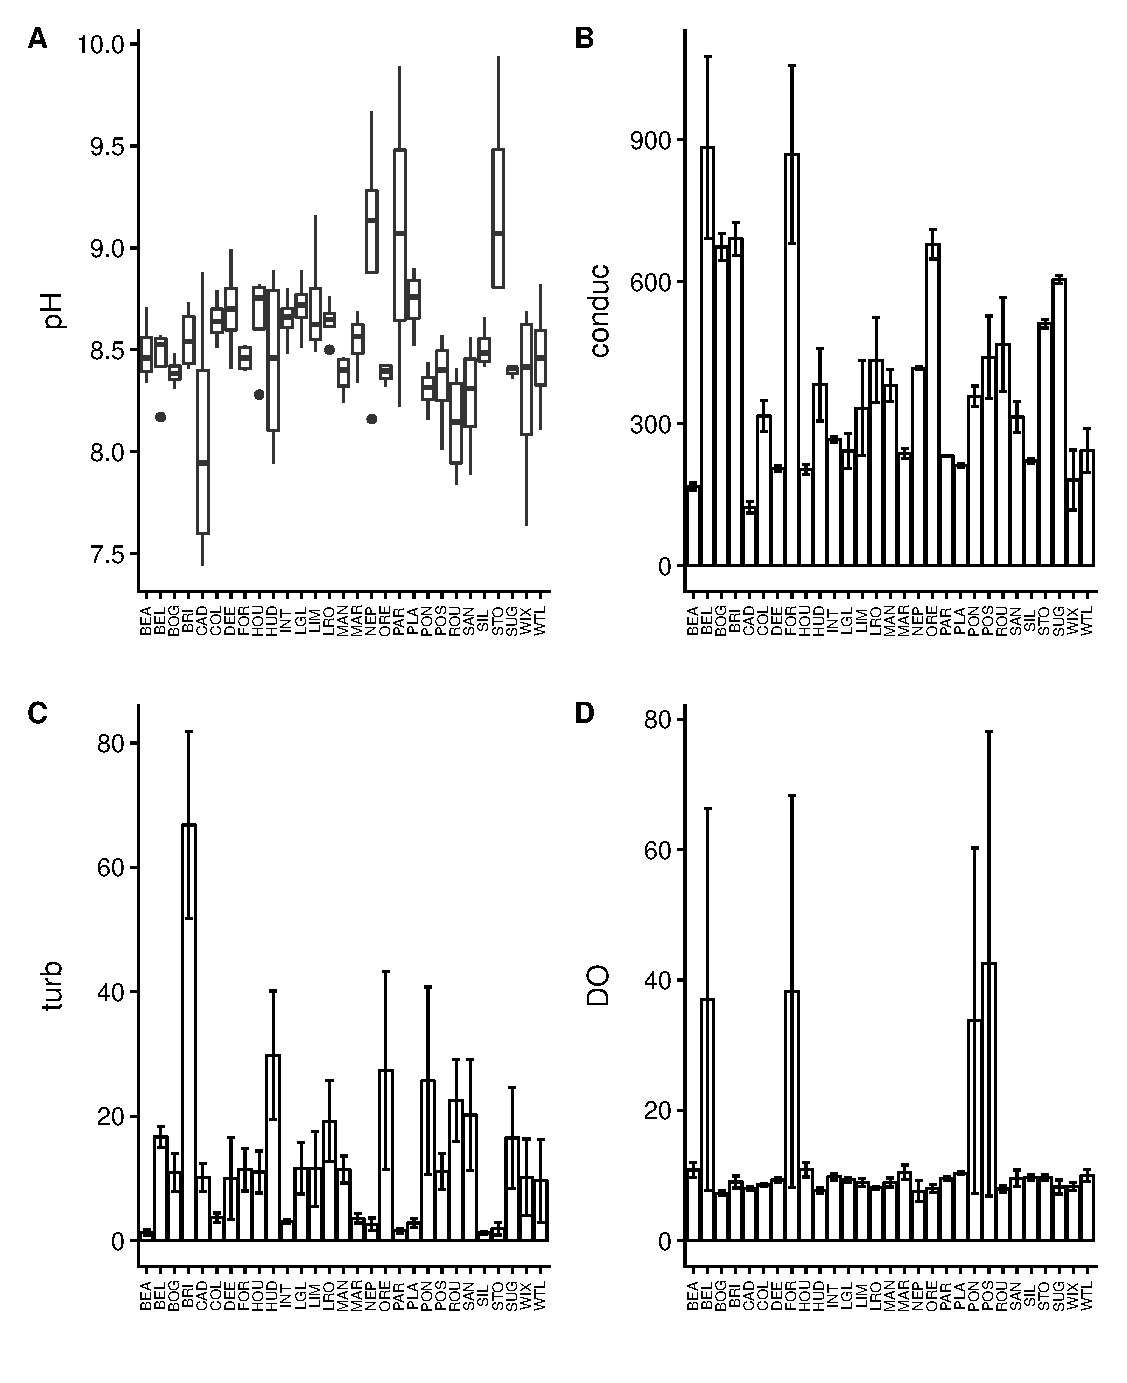
\includegraphics[width=\textwidth]{figures/watboxplotlake.eps}
\caption{Summary of measured water chemical parameters. Figure (A): A box and whisker plot of pH. Figure (B): Bar plots of average conductance. Figure (C): Average turbidity. Figure(D): Average dissolved oxygen. }
  \end{figure}
